\documentclass[floatfix,nofootinbib,superscriptaddress,fleqn]{revtex4-2}  
%\documentclass[aps,epsfig,tightlines,fleqn]{revtex4}
\usepackage[utf]{kotex}
\usepackage[HWP]{dhucs-interword}
\usepackage[dvips]{color}
\usepackage{graphicx}
\usepackage{bm}
%\usepackage{fancyhdr}
%\usepackage{dcolumn}
\usepackage{defcolor}
\usepackage{amsmath}
\usepackage{amsfonts}
\usepackage{amssymb}
\usepackage{amscd}
\usepackage{amsthm}
\usepackage[utf8]{inputenc}
 \usepackage{setspace}
 \usepackage{tikz}
%\pagestyle{fancy}

\begin{document}

\title{\Large 2022년 1학기 물리학 I: Quiz 17}
\author{김현철\footnote{Office: 5S-436D (면담시간 매주
    화요일-16:00$\sim$20:00)}} 
\email{hchkim@inha.ac.kr}
\author{Lee Hui-Jae} 
\email{hjlee6674@inha.edu}
\affiliation{Hadron Theory Group, Department of Physics,
Inha University, Incheon 22212, Republic of Korea }
\date{Spring semester, 2022}


\vspace{1.cm}

\maketitle


\noindent {\bf 문제 1. (40 pt)} 
태풍이 불 때 어떤 집의 지붕 위에서 바람(공기의 밀도 1.20 $\mathrm{kg/m^3}$)의
속력은 100 km/h였다.
\begin{itemize}
\item[(가)] 지붕의 안과 밖의 압력차는 얼마인가? 
\item[(나)] 지붕의 면적이 100 $\mathrm{m^2}$일 때, 바람이 지붕을
  들어올리는 힘은 얼마인가? 
 \end{itemize}

 \noindent {\bf 풀이 : } 
 \begin{itemize}
  \item[(가)] 
  지붕의 두께는 무시할 수 있을 정도로 작다고 가정하자.
  베르누이 방정식을 이용해 압력차를 구할 수 있다. 베르누이 방정식은
  \begin{align}
    P_1+\frac{1}{2}\rho v_1^2 +\rho gy_1
    =P_2+\frac{1}{2}\rho v_2^2 +\rho gy_2 
  \end{align}
  이다. 지붕의 두께를 $0$이라 하면 $y_1=y_2=0$이고 집 내부 공기가 
  일정한 방향으로 흐르지 않는다고 하면 $v_2=0$이다. 베르누이 방정식은
  다음과 같이 다시 쓸 수 있다.
  \begin{align}
    P_1+\frac{1}{2}\rho v_1^2
    =P_2.
  \end{align}
  $\rho$, $P_1$, $v_1$은 각각 공기의 밀도, 지붕 위에서 공기에 의한 압력,
  지붕 위에서 공기의 속력이다. $P_2$는 집 안에서 공기에 의한 압력이다. 따라서
  압력차 $\Delta P$는
  \begin{align}
    \Delta P = P_2 - P_1 = \frac{1}{2}\rho v_1^2
  \end{align}
  이다. 수치를 대입하면,
  \begin{align}
    \begin{split}
      \Delta P &= \frac{1}{2}(1.20\,\mathrm{kg/m^3}) (100\,\mathrm{km/h})^2
      = (0.60\,\mathrm{kg/m^3})
      \left(
        (100\,\mathrm{km/h})
        \left(\frac{1\,\mathrm{h}}{3\,600\,\mathrm{s}}\right) 
        \left(\frac{1\,000\,\mathrm{m}}{1\,\mathrm{km}}\right)
        \right)^2 \\
        &= 4.63\times 10^2\,\mathrm{N\cdot m^2}
      \end{split}
  \end{align}
  이다. 지붕의 안과 밖의 압력차는 $463\,\mathrm{N\cdot m^2}$이고 지붕 안의 압력이
  더 크다.
  \item[(나)] 
  지붕에 작용하는 힘은 지붕의 면적과 지붕에 작용하는 압력을 곱한 값과 같다. 
  지붕에 작용하는 총 압력은 아래로 작용하는 $P_1$과 위로 작용하는 $P_2$의 차이고
  이는 압력차 $\Delta P$와 같다.
  면적이 100 $\mathrm{m^2}$라면 지붕에 작용하는 힘은
  \begin{align}
    \begin{split}
      F &= \Delta P A = \frac{}{} \frac{1}{2}\rho v_1^2 A \\
      &= (0.60\,\mathrm{kg/m^3})
      \left(
        (100\,\mathrm{km/h})
        \left(\frac{1\,\mathrm{h}}{3\,600\,\mathrm{s}}\right) 
        \left(\frac{1\,000\,\mathrm{m}}{1\,\mathrm{km}}\right)
        \right)^2(100\,\mathrm{m^2})  \\
        &= 4.60\times 10^4\,\mathrm{N}
    \end{split}
  \end{align}
  이다. 압력은 위로 작용하므로 이 힘은 지붕을 들어올리는 힘이 된다.
 \end{itemize}

 \vspace{1.cm}

\noindent {\bf 문제 2. (60 pt)}
관의 지름이 $d$인 수도꼭지에서 물이 초기속도 $v$로 끊임없이 흘러나와서
아래로 떨어지고 있다(즉, 수도꼭지에서 나오는 물줄기의 지름이 $d$이고,
수도꼭지는 아래 방향을 향하고 있다). 수도꼭지에서 $h$만큼 떨어진 곳에서
물줄기의 지름은 얼마인가? 단, 공기의 저항은 무시하고, 물줄기는
끊어지거나 물방울이 되지 않는다고 가정한다.  
\begin{figure}[ht]
  \centering
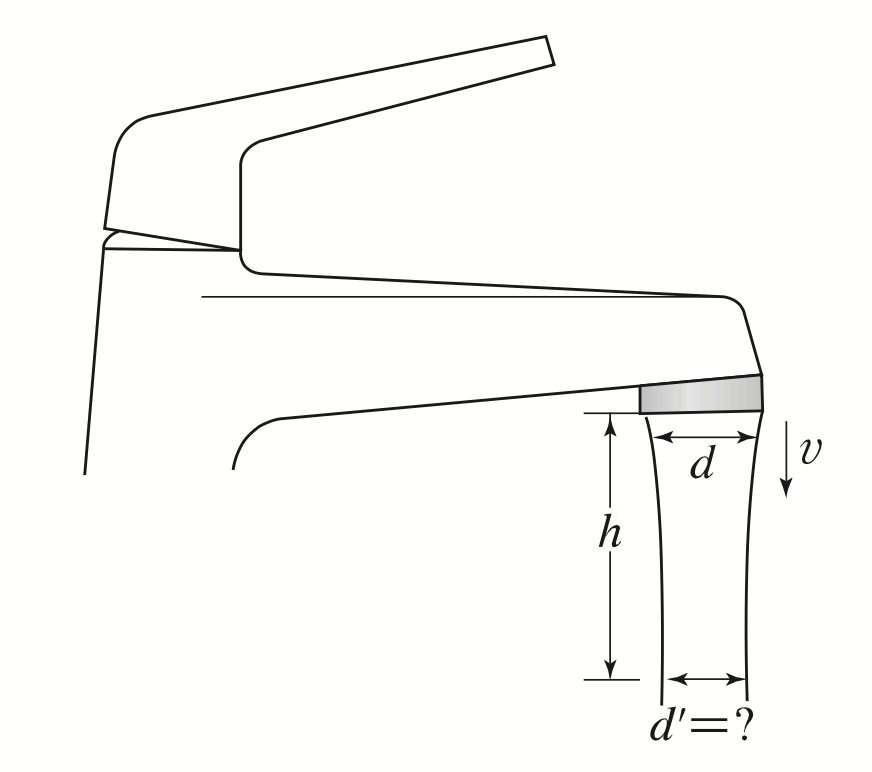
\includegraphics[scale=0.6]{Qfig17-1-20220509.png}
  \caption{문제 2}
  \label{fig:2}
\end{figure}

\noindent {\bf 풀이 : } 
관에서 나온 물에 대해 연속 방정식을 적용할 수 있다. 연속 방정식은
\begin{align}\label{eq:2-1}
  Av = A'v'
\end{align}
이다. $A$와 $v$는 관에서의 물줄기의 단면적과 속력이고 
$A'$와 $v'$는 $h$만큼 낙하한 물줄기의 단면적과 속력이다.
물은 낙하하면서 떨어진 높이만큼의 중력 퍼텐셜 에너지를 운동 에너지로 전환받으므로
\begin{align}\label{eq:2-2}
  \frac{1}{2}\rho v^2 = \frac{1}{2}\rho {v'}^2 + \rho g h
  \Longrightarrow {v'}^2 = v^2 + 2gh
\end{align} 
이다. 또한 $A$와 $A'$는 단면적이므로
\begin{align}\label{eq:2-3}
  A = \pi {\left(\frac{d}{2}\right)}^2,\,\,\,
  A' = \pi {\left(\frac{d'}{2}\right)}^2
\end{align}
이다. 식~\eqref{eq:2-1}에 식~\eqref{eq:2-2},~\eqref{eq:2-3}을 대입하면
\begin{align}
  \pi {\left(\frac{d}{2}\right)}^2 v
  = \pi {\left(\frac{d'}{2}\right)}^2\sqrt{v^2 + 2gh}
\end{align}
이고 우리가 구하고자 하는 $d'$에 대해 정리하면 다음을 얻을 수 있다.
\begin{align}
  d' = d{\left(\frac{v^2}{v^2+2gh}\right)}^{\frac{1}{4}}.
\end{align}
\vspace{1.cm}
\noindent {\bf 문제 3. (50pt)  }
질량 0.500 kg인 물체가 가벼운 용수철(용수철 상수 $2.40\times 10^3$
N/m)에 매달려 마루 위에 있다. 용수철을 평형지점에서 8.00 cm 압축하였다가 
놓았을 때
\begin{itemize}
\item[(가)] 운동방정식을 세워라.
\item[(나)] 초기위상은 얼마인가?
\item[(다)] $t=0.25$ s일 때 물체의 위치를 구하여라.
\item[(라)] 이 계의 총 에너지를 구하여라.
\item[(마)] $x=+5.0$ cm와 $x=-5.0$ cm일 때의 속도를 각각 구하여라.
\item[(바)] 물체의 최대속도를 구하여라. 어느 지점에서 나타나는가?
 \end{itemize}

 \noindent {\bf 풀이 : } 
 \begin{itemize}
  \item[(가)] 
  용수철이 평행지점으로부터 $x$만큼 압축되거나 늘어나면 훅의 법칙에 의해 $kx$만큼의
  복원력이 평행지점 방향으로 작용한다. 따라서 운동방정식은
  \begin{align}
    ma = -kx
  \end{align} 
  이다. 혹은 다음과 같이 적을 수 있다.
  \begin{align}\label{eq:3-1}
    \frac{d^2x}{dt^2} = -\omega^2x,\,\,\,\omega^2 = \frac{k}{m}.
  \end{align}
  \item[(나)] 
  초기위상을 구하기 위해 식~\eqref{eq:3-1}의 해를 구해보자. $x$를 두번 미분해서
  $x$에 $-\omega^2$가 곱해진 형태를 얻는 $x$는 삼각함수 혹은 지수함수의 형태라고
  가정할 수 있다. 즉,
  \begin{align}
    x(t) 
    =c\cos(\omega t + \phi)
  \end{align}
  라고 가정할 수 있다. 해를 어떻게 구할 수
  있을지 다루어보자. 
  용수철을 평행지점에서 $A$만큼 압축하였다가 놓았다는 것은
  $t=0$일 때 $x(0)=A$이고 $x'(0)=0$이라는 뜻이다. 
  $x(0)=A$이므로 $c$는 $c= A/\cos\phi$이고 $x'(0)=0$이므로
  \begin{align}\label{eq:3-2}
    x'(0) = -\frac{A\omega}{\cos\phi}\sin\phi = 0
  \end{align}
  이다. 식~\eqref{eq:3-2}가 $0$이기 위해서는 $\phi=0$이어야 한다. 따라서 $x(t)$에
  대한 표현은
  \begin{align}\label{eq:x}
    x(t) = A\cos\omega t
  \end{align}
  이고 초기위상 $\phi$는 $0$이다.
  \item[(다)] 
  $A=8.00$ cm이고 $m=0.500$ kg, $k=2.40\times 10^3$ N/m이다. 
  $t=0.25$ s일 때 물체의 위치를 알고 싶으므로 수치들을
  식~\eqref{eq:x}에 대입하면
  \begin{align}
    \begin{split}
      x(0.25\,\mathrm{s}) &= (8.00\,\mathrm{cm})
      \cos\left(
        \sqrt{\frac{2.40\times 10^3\,\mathrm{N/m}}{0.500\,\mathrm{kg}}}
        (0.25\,\mathrm{s})\right) \\
        &=0.334\,\mathrm{cm}.
      \end{split}
  \end{align}
  이다. $t=0.25$ s일 때 물체의 위치는 평형점으로부터 $0.334\,\mathrm{cm}$만큼
  떨어진 곳이다.
  \item[(라)]
  계의 역학적 에너지를 구해보자. 식~\eqref{eq:x}으로부터
  탄성 퍼텐셜에너지 $E_p$와 운동에너지 $E_k$를 구할 수 있다.
  \begin{align}
    E_p = \frac{1}{2}kA^2\cos^2\omega t,\,\,\,
    E_k = \frac{1}{2}m\omega^2A^2\sin^2\omega t.
  \end{align}
  $m\omega^2=k$이므로 두 에너지의 합은
  \begin{align}
    E_p +  E_k = \frac{1}{2}kA^2(\cos^2\omega t+\sin^2\omega t)
    =\frac{1}{2}kA^2
  \end{align}
  이다. 따라서 $E_p$는
  \begin{align}
    \begin{split}
      E_p &= \frac{1}{2}kA^2 = \frac{1}{2}
      (2.40\times 10^3\,\mathrm{N/m})
      (8.00\times 10^{-2}\,\mathrm{m})^2  \\
      &= 7.68\,\mathrm{J}
    \end{split}
  \end{align}
  이다.

  \item[(마)] 
  식~\eqref{eq:x}으로부터,
  \begin{align}\label{eq:x'}
    x'(t) = -\omega A\sin\omega t = -\omega\sqrt{A^2-(x(t))^2}
  \end{align}
  이다. $x=+5.0$ cm와 $x=-5.0$ cm일 때 $x'(t)$는 
  \begin{align}
    \begin{split}
      x' &= -\left(
        \sqrt{\frac{2.40\times 10^3\,\mathrm{N/m}}{0.500\,\mathrm{kg}}}
        (0.25\,\mathrm{s})\right)
        \sqrt{(8.00\times 10^{-2}\,\mathrm{m})^2
        -(\pm 5.0\times 10^{-2}\,\mathrm{m})^2} \\
      1.1\,\mathrm{m/s}.
    \end{split}
  \end{align}
  이다. 이는 속력이 $1.1\,\mathrm{m/s}$임을 의미한다.
  \item[(바)] 
  식~\eqref{eq:x'}으로부터 물체의 속도는 
  $\omega t = \frac{3}{2}\pi,\,\frac{7}{2}\pi,\,\frac{11}{2}\pi,\,\cdots$
  일 때 최대이다. 즉, 물체의 속도가 최대가 되는 조건은
  \begin{align}
    \omega t = \frac{3}{2}\pi+2n\pi,\,\,\,n=0,1,2,3,\cdots
  \end{align}
  이다. 물론 물체의 속력만을 고려한다면 부호를 따지지 않아도 되기 때문에
  $\omega t = \frac{1}{2}\pi,\,\frac{5}{2}\pi,\,\frac{9}{2}\pi,\,\cdots$
  인 순간에도 속력이 최대가 된다. 속도가 최대일 때 물체의 위치 $x(t)$는 
  \begin{align}
    x(t) = A\cos\left(\frac{3}{2}\pi+2n\pi\right) = 0
  \end{align}
  이다. 따라서 물체의 속도가 최대일 때 물체는 항상 평형점에 위치한다.
 \end{itemize}



 \vspace{1.cm}
\noindent {\bf 문제 4. (40pt)}
그림~\ref{fig:4}와 같이 반지름이 $R$이고 질량이 $M$인 원판, 링, 속이
꽉 찬 공,속이 텅빈 공을 길이가 $L$인 질량을 무시할 수 있는 실에 매달아
각 $\theta$까지 들어올렸다가 단진동을 시킨다. 
\begin{figure}[ht]
  \centering
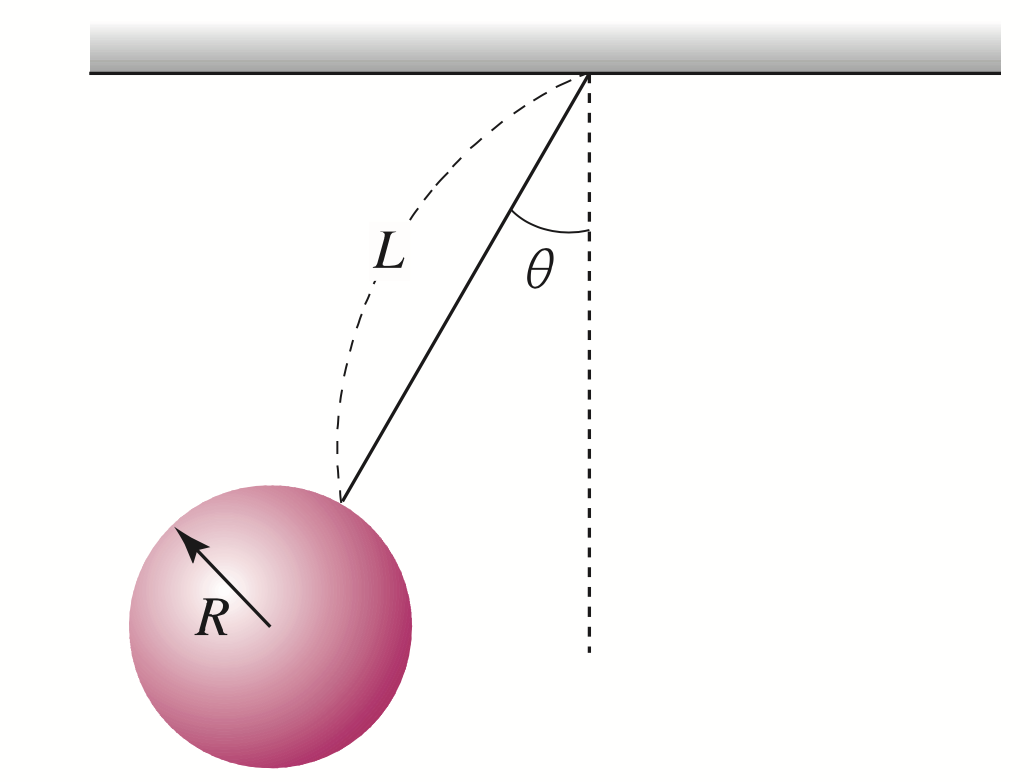
\includegraphics[scale=0.25]{Qfig17-4-20220509.png}
  \caption{문제 4}
  \label{fig:4}
\end{figure}
\begin{itemize}
\item[(가)] 단진동 주기가 가장 긴 것은 어느 것인가?
\item[(나)] 제일 아래 점에서 질량중심의 속력이 가장 큰 것은 어느 것인가?
\item[(다)] 이러한 진자를 달로 가져가서 똑같은 실험을 하면 주기는
  어떻게 되겠는가?
\item[(라)] 제일 아래 점에서 물체의 각속력을 $\omega$라 할 때 실의 장력은? 
\end{itemize}

\noindent {\bf 풀이 : } 
\begin{itemize}
  \item[(가)] 
  단진동 주기를 구하기 위해 진자의 운동방정식을 세워보자. 진자는 실과 벽이 연결된 지점을
  축으로 하여 회전운동 하는 것으로 생각할 수 있다. 이 때 진자에 대한 돌림힘 $\tau$는
  진자에 작용하는 중력으로부터 발생한다. 따라서 진자의 중심에 작용하는 돌림힘 $\tau$는
  \begin{align}\label{}
    \tau = -Mg\left(L+R\right)\sin\theta 
  \end{align}
  이다. 이 식은 $\theta\ll 1$이라고 근사하여 간단하게 풀 수 있다. $\theta\ll 1$이면
  $\sin\theta\approx\theta$이고 $\tau = I\alpha$이므로
  \begin{align}\label{}
    \tau = I\alpha = -Mg\left(L+R\right)\theta 
  \end{align}
  이고 이는 $\theta$에 대한 미분방정식이다.
  \begin{align}\label{}
    \frac{d^2\theta}{dt^2}=-\frac{Mg}{I}\left(L+R\right)\theta.
  \end{align}
  따라서 이 진자의 각진동수 $\omega$는
  \begin{align}\label{}
    \omega = \sqrt{\frac{Mg}{I}\left(L+R\right)}
  \end{align}
  이고 주기 $T$는
  \begin{align}\label{eq:4-T}
    T =\frac{2\pi}{\omega}= 2\pi\sqrt{\frac{I}{Mg}\left(\frac{1}{L+R}\right)}
  \end{align}
  이다. 주기가 회전관성 $I$에 의존하므로 각 경우에 대한 회전관성을 고려하여 주기를 구해보자.
  \begin{align*}
  \text{원판인 경우 : }         
   I= \frac{1}{2}MR^2 + M(L+R)^2\Longrightarrow&
   T = 2\pi\sqrt{\left(\frac{R^2}{2g}
   +\frac{(L+R)^2}{g}\right)\left(\frac{1}{L+R}\right)},\\
  \text{링인 경우 : }         
   I= MR^2 + M(L+R)^2 \Longrightarrow&          
  T = 2\pi\sqrt{\left(\frac{ R^2}{g}
  +\frac{(L+R)^2}{g}\right)\left(\frac{1}{L+R}\right)},\\
  \text{속이 꽉 찬 공인 경우 : }
   I= \frac{2}{5}MR^2 + M(L+R)^2 \Longrightarrow&
   T = 2\pi\sqrt{\left(\frac{2R^2}{5g}+\frac{(L+R)^2}{g}\right)
   \left(\frac{1}{L+R}\right)},\\
  \text{속이 텅 빈 공인 경우 : }
   I= \frac{2}{3}MR^2 + M(L+R)^2 \Longrightarrow&
   T = 2\pi\sqrt{\left(\frac{2R^2 }{3g}+\frac{(L+R)^2}{g}\right)
   \left(\frac{1}{L+R}\right)}.
  \end{align*}
  주기가 가장 긴 경우는 링인 경우이다.
  \item[(나)] 
  식~\eqref{eq:4-T}로부터 각진동수 $\omega$는 주기 $T$에 반비례함을 알 수 있다.
  (가)에서 주기가 가장 긴 경우는 링이고 가장 짧은 경우는 속이 꽉 찬 공임을 알 수 있으므로 
  각속도가 가장 큰 경우는 속이 꽉 찬 공이다.
  \item[(다)] 
  식~\eqref{eq:4-T}로부터 주기 $T$가 $\sqrt{1/g}$에 비례하므로
   중력가속도 $g$가 줄어들면 주기 $T$가 늘어남을 알 수 있다.
  달에서의 중력가속도 $g_m$은 지구에서의 중력가속도 $g$의 1/6배이므로 달에서의 주기를
  $T_m$이라 하면
  \begin{align}
    T_m = 2\pi\sqrt{\frac{6I}{Mg}\left(\frac{1}{L+R}\right)}=\sqrt{6}T
  \end{align}
  이다. 따라서 달에서의 주기는 지구에서의 주기의 $\sqrt{6}$배이다.
  \item[(라)] 


  \begin{figure}[htp]
    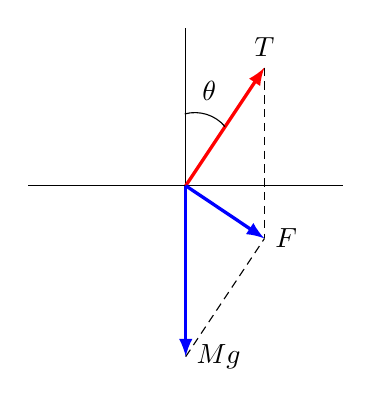
\begin{tikzpicture}
      \coordinate (T) at (1,1.5);
      \coordinate (G) at (0,-2.17);
      \coordinate (O) at (0,0);
      \coordinate (S) at (1,-0.67);
      \draw (-2,0) -- (2,0);
      \draw (0,-2) -- (0,2);
      \draw [red,very thick,-latex] (O) -- (T) 
      node [above,black] {$T$};
      \draw [blue,very thick,-latex] (O) -- (G) 
      node [right,black] {$Mg$};
      \draw [blue,very thick,-latex] (O) -- (S) 
      node [right,black] {$F$};
      \draw [densely dashed] (T) -- (S);
      \draw [densely dashed] (G) -- (S);
      \draw[] (0.5,0.75) arc(40:105:0.5) (0.3,1.2)
      node[] {$\theta$};
      \end{tikzpicture}
    \end{figure}

    장력 $T$를 구하기 위해 운동방정식을 세워보자. 다만 $x$, $y$축이 아니라 물체의 운동방향과
    그에 수직한 방향으로 성분을 나눌 것이다. 이는 물체의 회전축을 원점으로 하여 극좌표를 생각하는 것과 같다.
    물체의 운동방향 힘을 $F_{\theta}$,수직한 방향 힘을
    $F_r$이라고 하면 운동방정식은 다음과 같이 세울 수 있다.
    \begin{align}
      \label{eq:4-1}\sum F_r &= T - Mg\cos\theta = \frac{Mv^2}{L+R} ,   \\
      \label{eq:4-2}\sum F_{\theta} &=Ma_{\theta} =  Mg\sin\theta.
    \end{align}
    식~\eqref{eq:4-1}의 우변은 구심력이다. 속도는 각속도와 회전 반지름을 곱한 것이므로
    \begin{align}
      v = (L+R)\omega
    \end{align}
    이고 장력 $T$는 다음과 같다.
    \begin{align}
      T = Mg\cos\theta + M(L+R)\omega^2.
    \end{align}
\end{itemize}
\end{document}